\documentclass{ximera}

\author{Anna Davis} \title{MTH 160 Homework 6} 

\begin{document}

\begin{abstract}

\end{abstract}
\maketitle
 \textit{Certificate due: 10/7/2020 at 11:59 p.m.}
 \section{Lecture 13}
 
  \begin{problem}\label{prob:160hom6prob1} 
 A daycare center wishes to enclose a play area adjacent to the building, as shown in the diagram below.  If 200 linear feet of fencing is available, find the maximum possible area of the enclosure. 
 \begin{image}
   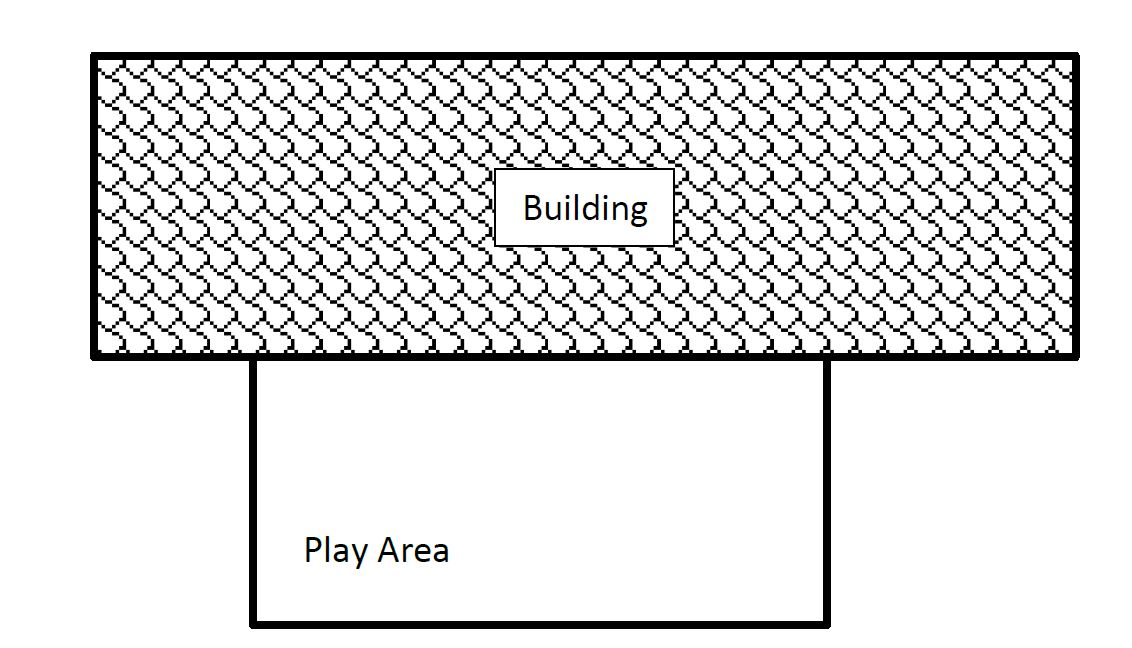
\includegraphics[height=1in]{160H6pic1.jpg}
 \end{image}
 Maximum possible area: $\answer{5000}$ sq. feet.
 \end{problem}
 
  \section{Lectures 14,15}
 
 \begin{problem}\label{prob:160hom6prob2} 
 For each given function, find all asymptotes and intercepts.   If the specified item does not exist, type DNE (case-sensitive) in the space provided.  
  \begin{enumerate}
\item
$f(x)=\frac{2x+3}{x-1}$

Horizontal Asymptote: $y=\answer{2}$

Vertical Asymptote: $x=\answer{1}$

$y$-intercept: $(0, \answer{-3})$

$x$-intercept: $(\answer{-\frac{3}{2}},0)$

\item
$f(x)=\frac{x-1}{x^2+10x-24}$

Horizontal Asymptote: $y=\answer{0}$

Vertical Asymptotes (from left to right): $x=\answer{-12}$, $x=\answer{2}$

$y$-intercept: $(0, \answer{\frac{1}{24}})$

$x$-intercept: $(\answer{1},0)$
\item
$f(x)=\frac{x}{x^2+9}$

Horizontal Asymptote: $y=\answer{0}$

Vertical Asymptote: $x=\answer{DNE}$

$y$-intercept: $(0, \answer{0})$

$x$-intercept: $(\answer{0},0)$

\item
$f(x)=\frac{x^2-1}{x-2}$

Horizontal Asymptote: $y=\answer{DNE}$

Vertical Asymptote: $x=\answer{2}$

$y$-intercept: $(0, \answer{\frac{1}{2}})$

$x$-intercepts (from left to right): $(\answer{-1},0)$, $(\answer{1},0)$
  \end{enumerate}
\end{problem}
 \end{document}